\documentclass{article}

\usepackage{graphicx}
\usepackage{tikz}
\usepackage{tikzsymbols}
\usetikzlibrary{calc,patterns,shapes.geometric}
\pagestyle{empty}
\usepackage[margin=0pt]{geometry}
\geometry{papersize={14in,12in}}

\def\centerarc[#1](#2)(#3:#4:#5){\draw[#1] ($(#2)+({#5*cos(#3)},{#5*sin(#3)})$) arc (#3:#4:#5);}

\begin{document}
	\begin{figure}
		\centering
		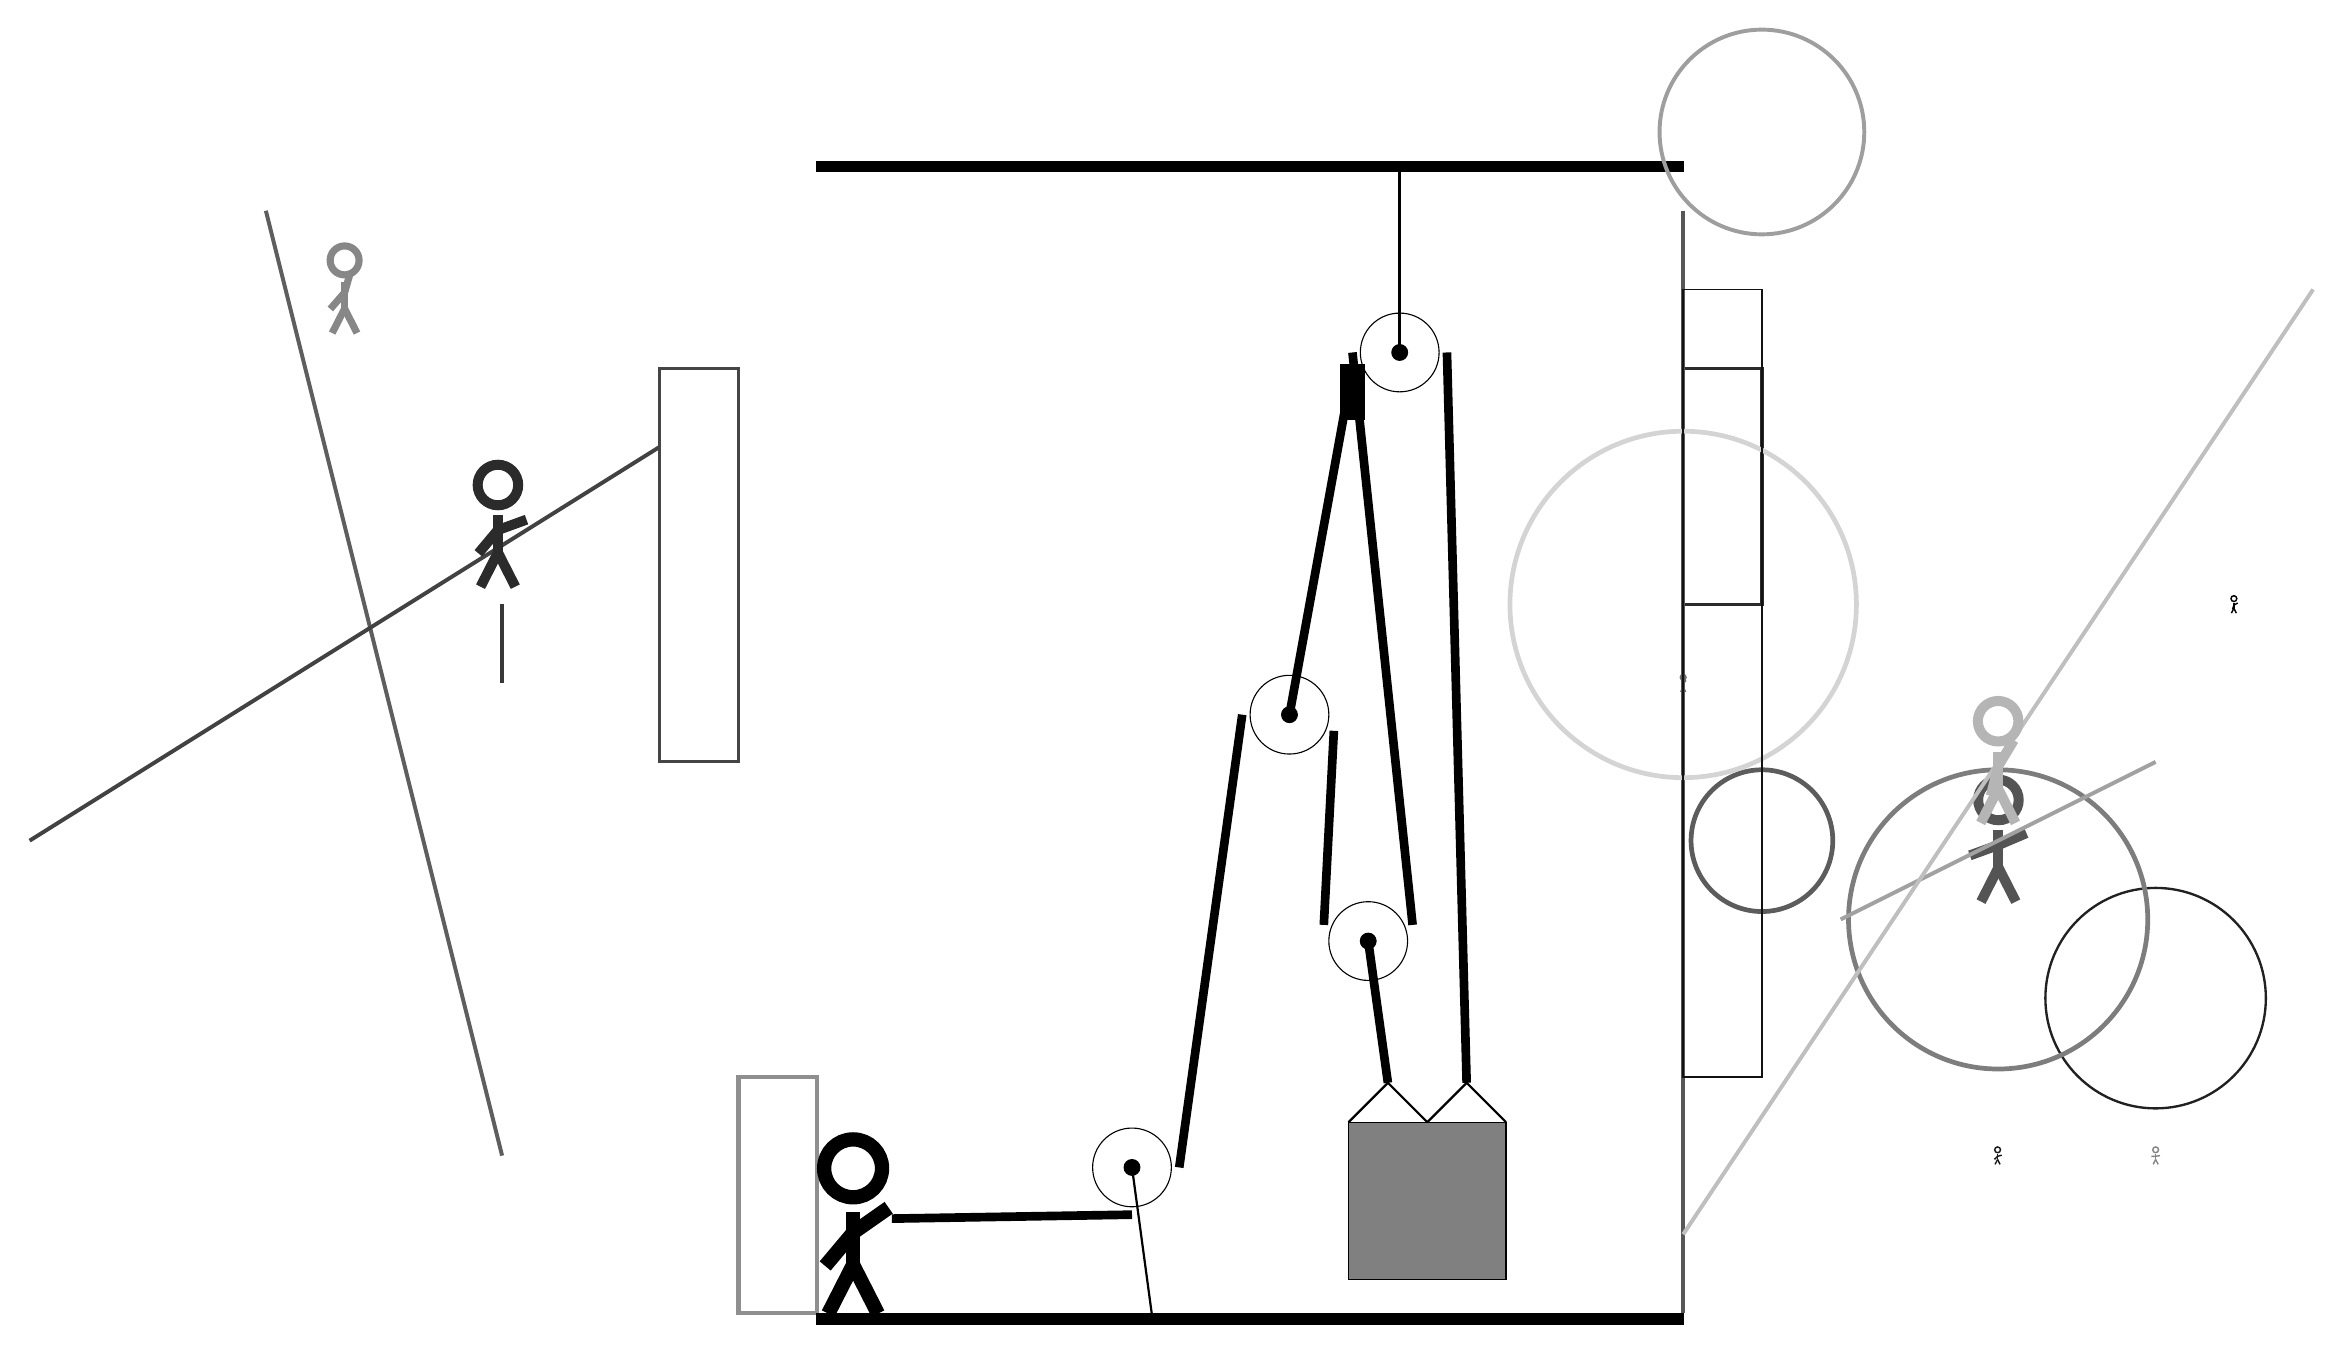
\begin{tikzpicture}
			%%%%% START %%%%%
			
			\draw[fill=black] (-6, 11.5) rectangle (5, 11.625);
			
			\draw (0, 4.6) circle (0.5);
			\draw[fill=black] (0, 4.6) circle (0.1);
			
			\node[line width=0.6mm, color=black!57] at (5, 5) {\Strichmaxerl[1][83][50]};
			
			\node[line width=0.6mm, color=black!67] at (9, 3) {\Strichmaxerl[7][20][23]};
			\draw[line width=0.2mm, color=black!69] (-7, 9) rectangle (-7, 9);
			\draw[line width=0.5mm, color=black!63](-10, -1) -- (-13, 11);
			
			\draw[line width=0.5mm, color=black!74](-8, 8) -- (-16, 3);
			
			\draw[line width=0.4mm, color=black!73] (-8, 4) rectangle (-7, 9);
			
			\node[line width=0.5mm, color=black!83] at (-10, 7) {\Strichmaxerl[7][50][20]};
			\draw [line width=0.6mm, color=black!64](6, 3) circle (0.9);
			\node[line width=0.6mm, color=black!90] at (9, -1) {\Strichmaxerl[1][44][14]};
			\node[line width=0.6mm, color=black!100] at (12, 6) {\Strichmaxerl[1][72][28]};
			\draw[line width=0.4mm, color=black!83] (5, 9) rectangle (6, 6);
			\draw[line width=0.5mm, color=black!66](5, 11) -- (5, -3);
			\draw [line width=0.6mm, color=black!17](5, 6) circle (2.2);
			
			\draw [line width=0.3mm, color=black!87](11, 1) circle (1.4);
			\draw [line width=0.5mm, color=black!38](6, 12) circle (1.3);
			\node[line width=0.5mm, color=black!48] at (11, -1) {\Strichmaxerl[1][3][8]};
			\draw [line width=0.6mm, color=black!51](9, 2) circle (1.9);
			\draw[line width=0.5mm, color=black!37](7, 2) -- (11, 4);
			\draw[line width=0.5mm, color=black!78](-10, 6) -- (-10, 5);
			
			\draw[line width=0.5mm, color=black!25](5, -2) -- (13, 10);
			\draw[line width=0.6mm, color=black!44] (-6, 0) rectangle (-7, -3);
			\draw[line width=0.2mm, color=black!93] (5, 0) rectangle (6, 10);
			\node[line width=0.5mm, color=black!47] at (-12, 10) {\Strichmaxerl[5][49][74]};
			\node[line width=0.3mm, color=black!29] at (9, 4) {\Strichmaxerl[7][76][59]};
			
			\draw (1, 1.725) circle (0.5);
			\draw[fill=black] (1, 1.725) circle (0.1);
			
			\draw (1.4, 9.2) circle (0.5);
			\draw[fill=black] (1.4, 9.2) circle (0.1);
			\draw[very thick] (1.4, 9.2) -- (1.4, 11.5);
			
			\draw (-2, -1.15) circle (0.5);
			\draw[fill=black] (-2, -1.15) circle (0.1);
			\draw[thick] (-2, -1.15) -- (-1.75, -3);
			
			
			\draw[thick]  (0.75, -0.575) -- (1.25, -0.075) -- (1.75, -0.575) -- (2.25, -0.075) -- (2.75, -0.575);
			\draw[fill=black!50] (0.75, -0.575) rectangle (2.75, -2.575);
			\draw[line width=1.1mm] (-5.05, -1.8) -- (-2, -1.75);
			\centerarc[line width=1.1mm](-2, -1.15)(270:360:0.6);
			\draw[line width=1.1mm] (-1.4, -1.15) -- (-0.6, 4.6);
			\draw[line width=1.1mm] (0, 4.6) -- (0.8, 9.0);
			\draw[line width=1.1mm, fill=black](0.7, 8.4) rectangle (0.9, 9.0);
			\centerarc[line width=1.1mm](0, 4.6)(-20:180:0.6);
			\draw[line width=1.1mm] (0.5638, 4.3948) -- (0.4362, 1.9302);
			\centerarc[line width=1.1mm](1, 1.725)(160:380:0.6);
			\draw[line width=1.1mm] (1.5638, 1.9302) -- (0.8, 9.2);
			\draw[line width=1.1mm](1, 1.725) -- (1.25, -0.075);
			\centerarc[line width=1.1mm](1.4, 9.2)(0:180:0.6);
			\draw[line width=1.1mm] (2.0, 9.2) -- (2.25, -0.075);
			
			\node at (-5.5, -1.9) {\Strichmaxerl[10][50][35]};
			
			\draw[fill=black] (-6, -3) rectangle (5, -3.15);
			
			%%%%% END %%%%%
		\end{tikzpicture}
	\end{figure}	
\end{document}